%% State Space Modelling of Dynamic Systems
%% Lecture 21: State Observers
\def\FileDate{10/04/02}
\def\FileVersion{1.0}
% ----------------------------------------------------------------
% Notes pages *********************************************************
% ----------------------------------------------------------------

In many practical cases it is not possible to measure all the states of a system.
That is  we cannot form  $u=r-\mathbf{Kx}$  for the purposes of feedback control because we do not have access to $\mathbf{x}$\footnote{Or some states in $\mathbf{x}$, either because the states are not \emph{physical states} and hence cannot be measured, or because they \emph{are} physical states but we do not have suitable sensors for the physical quantity that is represented by the state.}

If the structure of the system is known  (i.e. $\mathbf{A}$, $\mathbf{B}$, $\mathbf{C}$, and $\mathbf{D}$) then it may be possible to reconstruct the states from one or more of the system outputs by means of an observer. It is necessary that the system states be observable from the output(s).

\ifslidesonly
\begin{slide}
   \heading{State Observers}
   \begin{itemize}
   	\item In many practical cases it is not possible to measure all the states of a system.
   	\item That is  we cannot form  $u=r−\mathbf{Kx}$  for the purposes of feedback control because we do not have access to $\mathbf{x}$.
   	\item If we know $\mathbf{A}$, $\mathbf{B}$, $\mathbf{C}$, and $\mathbf{D}$ then it may be possible to reconstruct the states from one or more of the system outputs by means of an \textbf{observer}. 
   	\item It is necessary that the system states be observable from the output(s).
   \end{itemize}
\end{slide}
\fi

\begin{slide}
   \heading{State Observer}
The main idea is to construct a model of the system and subject it to the same input:
\begin{center}
	\resizebox{200pt}{!}{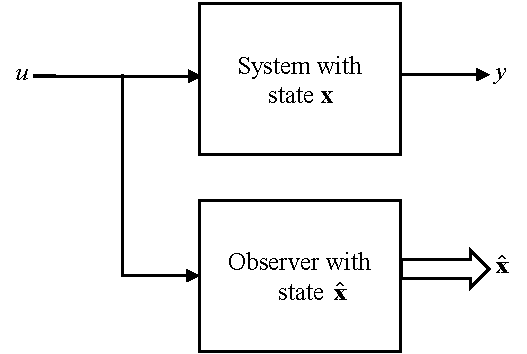
\includegraphics{pictures/observer1.pdf}}
\end{center}
\end{slide}

Severe differences occur between $\mathbf{x}$  and  $\hat{\mathbf{x}}$ due to disturbances and parameter errors. Solution:-  Employ feedback !

\begin{slide}
   \heading{State Observer with Feedback}
\begin{center}
	\resizebox{280pt}{!}{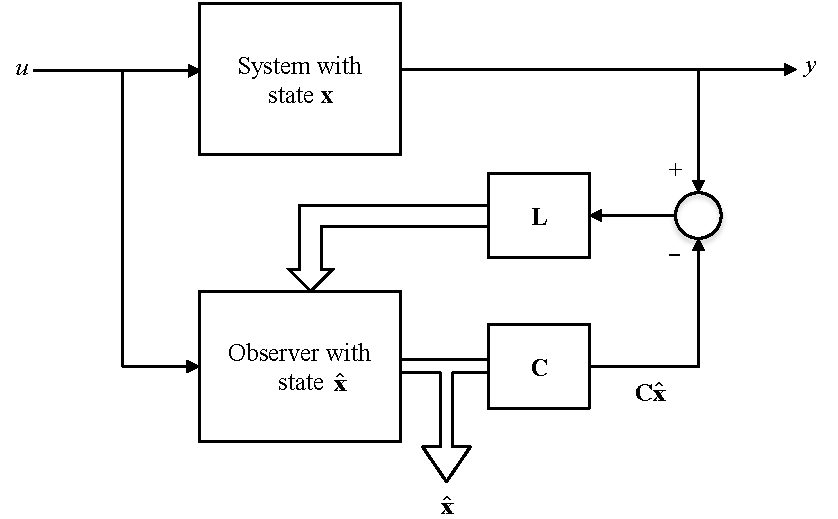
\includegraphics{pictures/observer2.pdf}}
\end{center}
\end{slide}
\textbf{NB} To simplify treatment, we take $\mathbf{D}=0$.

For the \textbf{observer} we have the state equations:
\[
\frac{{d{\bf{\hat x}}}}{{dt}} = {\bf{A\hat x}} + {\bf{B}}u + {\bf{L}}\underbrace {(y - {\bf{C\hat x}})}_{{\rm{feedback}}}
\]

Let the error in the estimated states $\hat{\mathbf{x}}$ be:
\[
\mathbf{e}=\mathbf{x}=\hat{\mathbf{x}}
\]
then
\[
\frac{d\mathbf{e}}{dt}=\frac{d\mathbf{x}}{dt}-\frac{d\hat{\mathbf{x}}}{dt}
\]

Given,
\[
\frac{d\mathbf{x}}{dt}=\mathbf{A}\mathbf{x}+\mathbf{B}u\ \mathrm{and}\ y=\mathbf{C}\mathbf{x}
\] 
then
\begin{eqnarray*}
	\frac{d\mathbf{e}}{dt} & = & \left(\mathbf{A}\mathbf{x}+\mathbf{B}u\right)-\left\{\mathbf{A}\hat{\mathbf{x}}+\mathbf{B}u+\mathbf{L}(y-\mathbf{C}\hat{\mathbf{x}})\right\} \\
	& = & \mathbf{A}(\mathbf{x}-\hat{\mathbf{x}})-\mathbf{L}(\mathbf{C}\mathbf{x}-\mathbf{C}\hat{\mathbf{x}}) = \mathbf{Ae}-\mathbf{LCe}\\
	& = & (\mathbf{A}-\mathbf{LC})\mathbf{e}
\end{eqnarray*}
 
\begin{itemize}
	\item These are the state equations for the observer error.
	\item The errors decay to zero with time if the eigen values of  $(\mathbf{A}−\mathbf{LC})$ lie in the left half plane (LHP).
	\item In fact we can design the matrix $\mathbf{L}$ to place the eigen values anywhere we wish
	\item If we place them well into the LHP then $\mathbf{e}$ will decay quickly to zero making the observer states accurately track the system states $\mathbf{x}$ after a short time.
	\item $\hat{\mathbf{x}}$ can then be used for feedback control.
\end{itemize}

\section*{Design of the $\mathbf{L}$ Matrix} % (fold)
\label{sec:design_of_the_l_matrix}

This is particularly easy when we use the observer canonical form:

Given the TF:
 

the matrices of the state space model are:

 
and the feedback vector is:
 
The state matrix of the observer is:
 
 
The poles of the observer are the roots of the CE:

 

If the desired observer poles are at  
then the desired CE equation is:

 

The  l  coefficients may be found by matching the two equations above:

Thus,

 


% section design_of_the_l_matrix (end)


\section*{Design of $\mathbf{L}$ Matrix for Other Forms of State Equation} % (fold)
\label{sec:design_of_l_matrix_for_other_forms_of_state_equation}


When the observer canonical form is not used, then the design of the observer is more difficult. Ackermann's formula can be adapted as follows:

 

O is the observability matrix:
 

 

Notice that if the system is unobservable, then the matrix inverse does not exist and we cannot design an observer for this system.

In MATLAB we could evaluate the L matrix using:

L=(acker(A',C',p))'  where  p  is a vector of desired observer poles.
 
eg.  Design an observer with poles or eigen values
–20,−20 using the observer canonical form for the system with a TF:
 
Answer:

The observer canonical form gives:

 

with     we have observer poles at the roots of:

 

The desired CE is:

 

 
Comparing coefficients gives:

 

So the observer states are given by:

 

Block Diagram of the Observer






% section design_of_l_matrix_for_other_forms_of_state_equation (end)








 
\section*{Choice of Observer Poles} % (fold)
\label{sec:choice_of_observer_poles}


•	Rule of thumb:   observer poles can be faster than the controller poles (i.e. further from the origin) by a factor of 2 to 6. This makes the effect of the observer dynamics short-term and the overall response is dominated by the controller poles.

•	If noise/disturbance is present this has an effect on the choice:
 

In the error equation, the sensor noise is multiplied by L and the process noise is not. Therefore,

 
(i)  if  L  is very small, the effect of sensor noise  v  is removed but the observer is “slow” to respond, so that the error will not reject the effect of  w  very well.

(ii)	if  L  is large, the observer response is “fast” and the error rejects the process noise  w  well, but the sensor noise  v  is amplified by  L  resulting in large errors.

Optimal control design methods can be used to achieve the “best” compromise.

% section choice_of_observer_poles (end)



%----------------------------------------------------------------
% The end of notes
% ----------------------------------------------------------------
\endinput

%%% Local Variables: 
%%% mode: latex
%%% TeX-master: t
%%% End: 
